\chapter{Planificación y costes}

%Definir claramente de acuerdo con el tutor los “paquetes de trabajo” (PTs), identificando claramente los entregables resultantes de cada uno de ellos. Esto definirá claramente los resultados del proyecto. Pueden usarse Diagramas de Gantt o cualquier herramienta o metodología siempre que facilite la visualización secuencial y dependencias entre los PT. En este mismo capítulo se incluir un presupuesto –ajustado en lo posible a la realidad- que incluya recursos humanos y materiales, así como cualquier dato que determine la viabilidad del proyecto.

En este capítulo se van a definir las diferentes etapas del proyecto mediante diagramas de Gantt realizados con la aplicación \textit{OpenProj}. Además se incluye el presupuesto necesario para la realización de dicho proyecto.

\section{Planificación}

La figura \ref{fig:gantt-ini} muestra la propuesta inicial de las etapas del proyecto, donde se diferencian varios bloques, el primero sería el de estudio e introducción a lo que se va a realizar en el proyecto, que comprendería desde septiembre hasta finales de noviembre, el segundo bloque o implementación del algoritmo, desde mediados de noviembre hasta finales de diciembre, el tercer bloque contiene todo lo referente a la \textit{blockchain} ARK siendo el grueso del proyecto, comienza a finales de enero hasta mayo. Y por último la parte de las de las pruebas, son 10 días en mayo. La memoria se ha redactado durante todo el proyecto.

\begin{figure}[h]
	\centering
	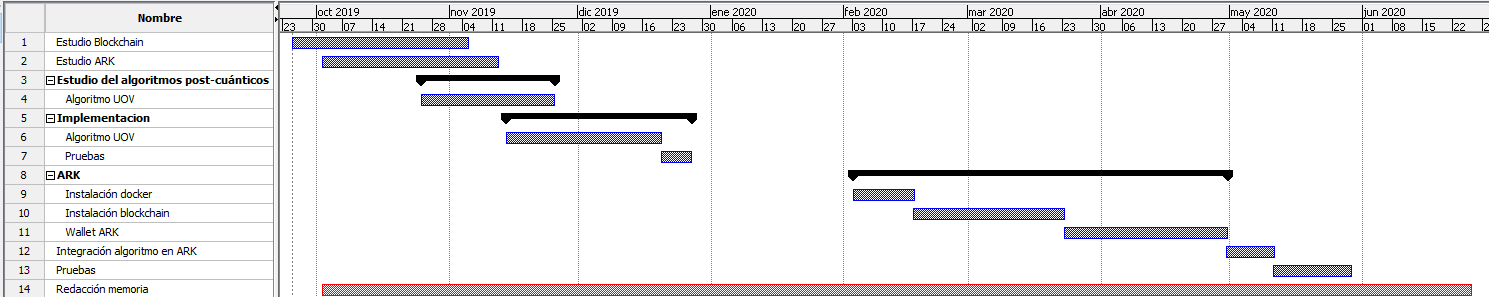
\includegraphics[width=15cm,height=5cm]{figuras/Gantt_ini.png}
	\caption{Digrama de Gantt inicial}
	\label{fig:gantt-ini}
\end{figure}

Pero no todo ha sido como se había planificado, puesto que han surgido algunos imprevistos. A la hora de realizar la implementación del algoritmo UOV en \texttt{python} no existe una biblioteca para trabajar con matrices y cuerpos finitos al mismo tiempo, así ha aumentado el tiempo que se iba a dedicar al algoritmo. Además el trabajo con ARK ha sido más tedioso del esperado, retrasando los tiempos programados.

El diagrama de Gantt real se ha dividido en partes para que se visualice mejor, la imagen \ref{fig:gantt-real-1} muestra las fases de estudio e implementación, la imagen \ref{fig:gantt-real-2} incluye el tiempo dedicado al trabajo con ARK hasta julio y la imagen \ref{fig:gantt-real-3} desde julio hasta noviembre, además del periodo de pruebas.


\begin{figure}[h]
	\centering
	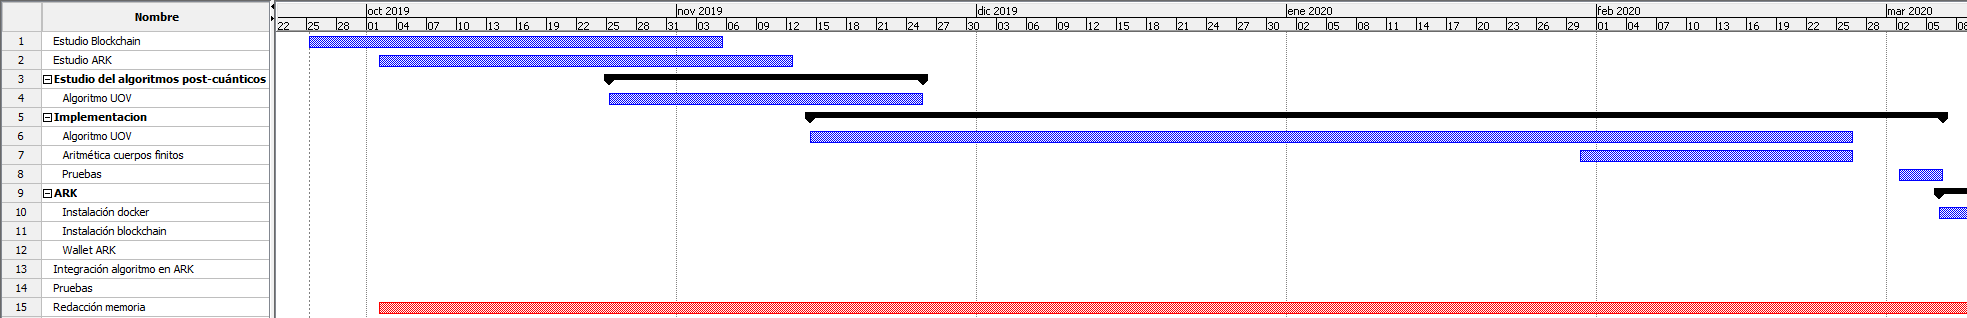
\includegraphics[width=15cm,height=6cm]{figuras/Gantt_1.png}
	\caption{Diagrama de Gantt real. Parte I}
	\label{fig:gantt-real-1}
\end{figure}

\begin{figure}[h]
	\centering
	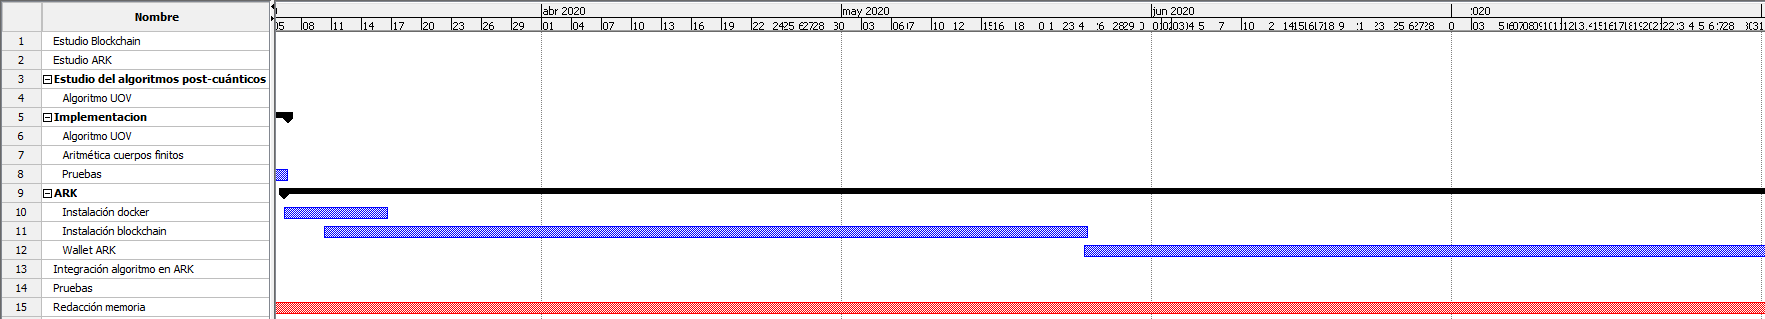
\includegraphics[width=15cm,height=6cm]{figuras/Gantt_2.png}
	\caption{Diagrama de Gantt real. Parte II}
	\label{fig:gantt-real-2}
\end{figure}

\begin{figure}[h]
	\centering
	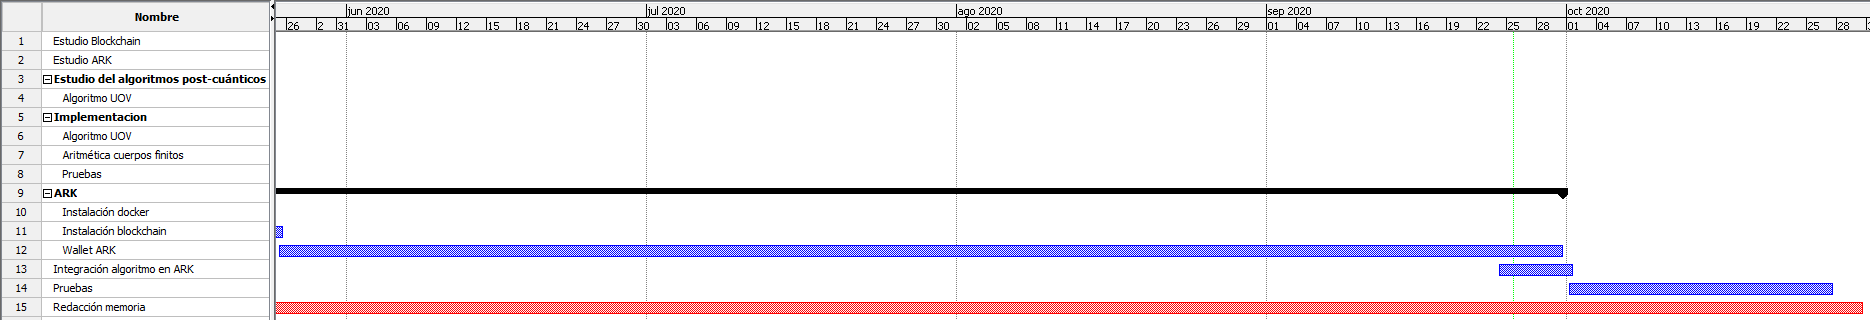
\includegraphics[width=15cm,height=6cm]{figuras/Gantt_3.png}
	\caption{Diagrama de Gantt real. Parte III}
	\label{fig:gantt-real-3}
\end{figure}

\section{Costes}

A continuación se va a detallar el presupuesto invertido en el desarrollo del proyecto. Se van a desglosar los costes en recursos humanos, inventariales, indirectos y viajes.

La tabla \ref{tab:coste-rh} muestra los costes de recursos humanos inclyen los tiempos deciados tanto al estudio como a la implementación y la redacción de la memoria. El precio estimado por cada hora de trabajo es de 12\euro.

\begin{table}[h]
	\label{tab:coste-rh}
	\begin{center}
	\centering
	\resizebox{\linewidth}{!}{
	\begin{tabular}{p{0.6\linewidth} p {0.15\linewidth}p{0.15\linewidth}}
		\textbf{Descripción del coste} & \textbf{Cantidad (horas)} & \textbf{Coste total (\euro)} \\
		\toprule
		Bloque de estudio\\
		\toprule
		Estudio tecnología blockchain & 32 & 384\\[0.5ex]
		Estudio ARK & 50 & 600\\
		Estudio algoritmo post-cuánticos & 28 & 336\\[0.5ex]
		\toprule
		Bloque de implementación\\
		\toprule
		Algoritmo UOV & 15 & 180\\[0.5ex]
		Aritmetica cuerpos finitos & 23 & 276\\[0.5ex]
		\toprule
		Bloque general\\
		\toprule
		Redacción memoria & 67 & 804\\[0.5ex]
		Corrección memoria & 19 & 228\\[0.5ex]
		Reuniones & 35 & 420\\[0.5ex]
		\bottomrule
		TOTAL (\euro) &\\
	\end{tabular}}
	\end{center}
	\caption{Desglose de los costes en recursos humanos}
\end{table}

El equipo de trabajo ha sido con un ASUS TP$300$L, teniendo en cuenta que el precio de adquisición del ordenador fue de $750,00$\euro\ y suponiendo que la vida media de un ordenador es de unos 6 años, entonces el gasto que corresponde durante los 13 meses del desarrollo del proyecto es de  $135,41$\euro.

En los costes indirectos se va a introducir la electricidad, material de oficina y servicio de mantenimiento. Este último incluye el precio de un nuevo disco de memoria interno, ya que ha sido necesario aumentar la memoria del portátil, veáse la tabla \ref{tab:coste-indi}.

\begin{table}[h]
	\label{tab:coste-indi}
	\begin{center}
	\centering
	\begin{tabular}{p{0.4\linewidth} p {0.2\linewidth}}
		\textbf{Descripción del coste} & \textbf{Cantidad} \\
		\toprule
		Electricidad & 100\euro\\[0.5ex]
		Material de oficina & 30\euro\\[0.5ex]
		Servicio de mantenimiento & 45\euro\\[0.5ex]
		\bottomrule
		TOTAL (\euro) & 175 \euro\\
	\end{tabular}
	\end{center}
	\caption{Desglose de los costes indirectos}
\end{table}

Por último tenemos los costes en viajes a la escuela de informática para las reuniones con el tutor, puesto que a la facultad de ciencias no era necesario coger un transporte. Solo se han realizado viajes en el primer cuatrimestre del curso $2019$-$2020$, ya que el resto de las reuniones han sido de forma virtual, obteniendo un total de costes de $12$\euro.


\begin{table}[h]
	\label{tab:coste-total}
	\begin{center}
	\centering
	\begin{tabular}{p{0.4\linewidth} p {0.2\linewidth}}
		\textbf{Tipo de costes} & \textbf{Cantidad} \\
		\toprule
		Recursos humanos & \\[0.5ex]
		Inventariales & 135.41\euro\\[0.5ex]
		Indirectos & 175\euro\\[0.5ex]
		Viajes & 12\euro\\[0.5ex]
		\bottomrule
		TOTAL (\euro) & \euro\\
	\end{tabular}
	\end{center}
	\caption{Presupuesto total desglosado}
\end{table}

Una vez que hemos calculado todos los gastos posibles, tabla \ref{tab:coste-total}, vamos a añadir un margen de contingencia del $5\%$ para posibles imprevistos del proyecto. Hemos obtenido que los gastos previstos serán de \euro, por tanto el margen de contigencia será de \euro, así el presupuesto final sera de \euro.